\documentclass{standalone}
\usepackage[dvipsnames]{xcolor}
\usepackage{tikz}
\usetikzlibrary{positioning,calc,fit
  ,matrix}


\definecolor{mybluei}{RGB}{124,156,205}
\definecolor{myblueii}{RGB}{73,121,193}
\definecolor{mygreen}{RGB}{202,217,126}
\definecolor{mypink}{RGB}{233,198,235}


\pgfdeclarelayer{background}
\pgfsetlayers{background,main}

\pgfkeys{
  /tikz/node distance/.append code={
    \pgfkeyssetvalue{/tikz/node distance value}{#1}
  }
}




\tikzset{
tikzcomputerpic/.style={ 
  node distance=20pt
    ,inner sep=0pt
    ,outer sep=0pt
}
,title/.style={ inner sep=0pt, color=white}
,bounder/.style={rounded corners,draw=black,inner sep=5pt}
,computer/.style={bounder}
,computername/.style={font=\sffamily\color{black}
  ,above=20pt of stack}
,blueb/.style={
  draw=white, line width=.5pt,
  fill=myblueii,
  text width=2.6cm,
  font={\sffamily\color{white}},
  align=center,
  text height=12pt,
  text depth=9pt
}
,span/.style={inner sep=0pt,text height=12pt}
,dockerapp/.style={blueb,fill=mybluei,font={\sffamily\bfseries\color{white}}}
,docker/.style={blueb,fill=myblueii}
,os/.style={blueb,fill=BurntOrange,font={\sffamily\color{black}}}
,stack/.style={ column sep=0em, row sep=0em}
,sharestyle/.style={blueb,fill=Aquamarine}
,app/.style={blueb,fill=Periwinkle}
}







\begin{document}

\newcommand\shareblock[2][\texttt{/project}]{
\node[sharestyle] (#2) {#1};
}

\begin{tikzpicture}[
node distance=4in
,inner sep=0pt
]


\node (vagrant) {
\begin{tikzpicture}[tikzcomputerpic]
%vagrant compute computer
 \matrix[stack](stack){
   \node[dockerapp] (vagapp1) {app1}; 
   & \node[dockerapp] (vagapp2) {app2}; 
   \\
  \node[dockerapp] (vaglib1) {};
  & \node[dockerapp] (vaglib2) {};
  & \node[dockerapp] (vagapp3) {app3}; 
  \\
  \node[docker] (vagdkr1) {};
  & \node[docker] (vagdkr2) {};
  & \node[docker] (vagdkr3) {};
  \\
  \node[sharestyle] (vagshare1) {};
  & \node[sharestyle] (vagshare2) {};
  & \node[sharestyle] (vagshare3) {};
  \\
  \node[os] (vagos1) {};
  & \node[os] (vagos2) {};
  & \node[os] (vagos3) {};
  \\
 };


%span is last
\node[dockerapp,fit= (vaglib1) (vaglib2),span] (vaglib) {lib};
\node[sharestyle,fit= (vagshare1) (vagshare2)(vagshare3),span]
(vaglib) {\texttt{/project}};
\node[docker,fit=(vagdkr1)(vagdkr2)(vagdkr3),span ] (vagdkr) {Docker}; \\
\node[os,fit=(vagos1)(vagos2)(vagos3),span ] (vagos) {CoreOS}; \\
\node[computername] (vagrantcomputenm) {``vagrant''};

\begin{pgfonlayer}{background}
 \node[computer
 ,fit=(vagrantcomputenm) (stack)] (vagrantcomputebox) {};
\end{pgfonlayer}
%Vagrant compute computer
\end{tikzpicture}
};




\node[left of=vagrant] (init) {
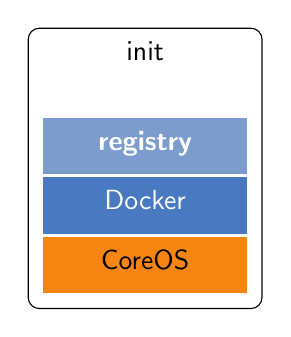
\begin{tikzpicture}[tikzcomputerpic]
  % init computer
  \matrix[stack](stack){
    \node[dockerapp] (initreg) {registry};
    \\
    \node[docker] (initdkr) {Docker}; 
    \\
    \shareblock{initshare};
    \\
    \node[os] (initos) {CoreOS}; 
    \\
  };
  \node[computername] (initnm) {init};
  \begin{pgfonlayer}{background}
    \node[computer,fit=(initnm) (stack)] (initbox) {};
  \end{pgfonlayer}
  % init computer
\end{tikzpicture}
};


\node[below of=vagrant] (local) {
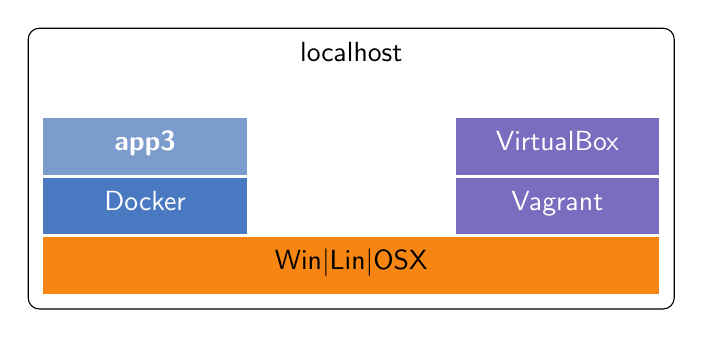
\begin{tikzpicture}[tikzcomputerpic]
  % local computer
  \matrix[stack](stack){
    \node[dockerapp] (localapp3) {app3}; 
    &
    & \node[app](localvirtualbox) {VirtualBox};
    \\
    \node[docker] (localdkr) {Docker};
    &   \shareblock[share:\texttt{/project}]{localshare}
    & \node[app](localvagrant) {Vagrant};
    \\
    \node[os] (localos1) {}; 
    & \node[os] (localos2) {}; 
    & \node[os] (localos3) {}; 
    \\
  };
\node[os,fit=(localos1)(localos2)(localos3),span]
(localos)
{Win\textbar Lin\textbar OSX}; 
  \node[computername] (localnm) {localhost};
  \begin{pgfonlayer}{background}
    \node[computer,fit=(localnm) (stack)] (localbox) {};
  \end{pgfonlayer}
\end{tikzpicture}
};


\node[right of=vagrant] (aws1) {
\begin{tikzpicture}[tikzcomputerpic]
%vagrant compute computer
 \matrix[stack](stack){
   \node[dockerapp] (aws1app1) {app1}; 
   & \node[dockerapp] (aws1app2) {app2}; 
   \\
  \node[dockerapp] (aws1lib1) {};
  & \node[dockerapp] (aws1lib2) {};
  & \node[dockerapp] (aws1app3) {app3}; 
  \\
  \node[docker] (aws1dkr1) {};
  & \node[docker] (aws1dkr2) {};
  & \node[docker] (aws1dkr3) {};
  \\
  \node[sharestyle] (aws1share1) {};
  & \node[sharestyle] (aws1share2) {};
  & \node[sharestyle] (aws1share3) {};
  \\
  \node[os] (aws1os1) {};
  & \node[os] (aws1os2) {};
  & \node[os] (aws1os3) {};
  \\
 };


%span is last
\node[dockerapp,fit= (vaglib1) (vaglib2),span] (vaglib) {lib};
\node[sharestyle,fit= (vagshare1) (vagshare2)(vagshare3),span]
(vaglib) {\texttt{/project}};
\node[docker,fit=(vagdkr1)(vagdkr2)(vagdkr3),span ] (vagdkr) {Docker}; \\
\node[os,fit=(vagos1)(vagos2)(vagos3),span ] (vagos) {CoreOS}; \\
\node[computername] (vagrantcomputenm) {aws1};

\begin{pgfonlayer}{background}
 \node[computer
 ,fit=(vagrantcomputenm) (stack)] (vagrantcomputebox) {};
\end{pgfonlayer}
%Vagrant compute computer
\end{tikzpicture}
};


\end{tikzpicture}

\end{document}